Stratum protocol, as we've seen, dramatically increased the performances of pooled mining operations, being effectively an efficient, robust, and scalable communication protocol.
It introduced a very different approach to pooled mining, giving the responsibility to drive the load and to distribute jobs for the miners to the mining pool operators.\\
By the way, it was developed in 2012: at that time the Bitcoin network difficulty was around 3.000.000 (global hashrate was 13 TH/s, at the time of writing it's 342 EH/s). As already said, the main purpose who took to the development of Stratum protocol, was to find a valid alternative to the previous getwork, given the fact that newest mining ASIC equipment was arriving at that time.\\
However, it's important to note that the security aspects of the Stratum protocol were not the primary focus during its development. At that time, the overall hashrate was relatively low compared to the present scenario, and considerations regarding encryption or secure communication were not extensively taken into account. As a result, the Stratum protocol was built with plaintext transmission for all protocol messages, without any encryption mechanisms to protect against potential security threats.

\subsubsection{Blackhat Asia 2021 - hashrate stealing attacks}
In 2021, during the Blackhat Asia event, a group of researchers (Xin Liu, Rui Chong, Yuanyuan Huang, Yingli Zhang, Qingguo Zhou) demonstrated how they succeeded in stealing some hashrate secretly, exploiting the plaintext communications present in the Stratum protocol \cite{blackhatasia}.\\
\begin{wrapfigure}{r}{0.45\textwidth}
    \centering
    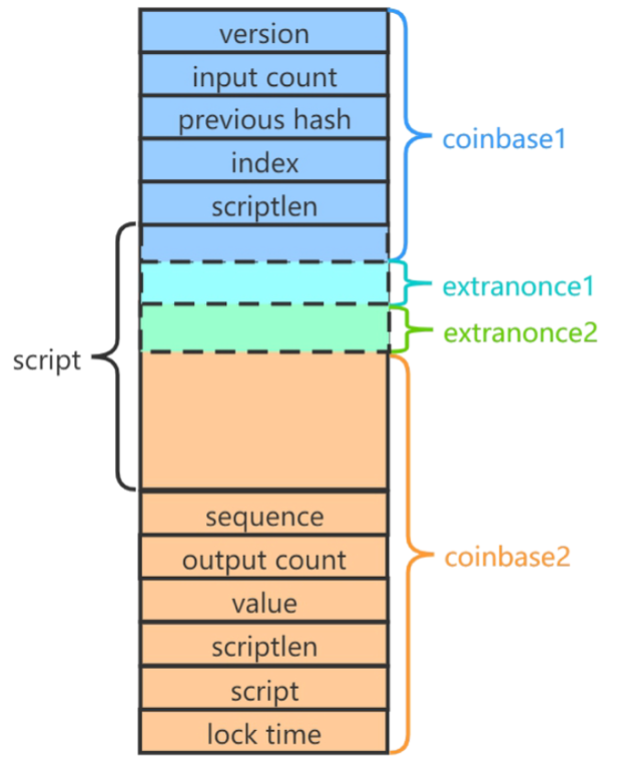
\includegraphics[width=0.30\textwidth]{Figures/stratum/stratum3.png}
    \caption{Coinbase tx details}
    \label{fig:stratum3}
\end{wrapfigure}
Before entering in the details of the two attacks which they discovered, a brief reminder of the \textbf{coinbase transaction} data, the \textbf{set.extranonce} message, and \textbf{client.reconnect} message is needed.\\
The coinbase transaction is not sent entirely by the mining pool server to the miner, but it's constructed by the miner once every needed information is received.
After the \textbf{subscription request} sent by the miner, the mining pool server answers with a message containing the \textbf{extranonce1} (which is different for every connection) and the \textbf{extranonce2 size}.
Using the \textbf{notify message}, instead, pool server sends to the miner the other components needed to build the entire coinbase transaction: the so called \textbf{coinbase1}, and \textbf{coinbase2} data.

\noindent The \textbf{set.extranonce} message, instead, it's used from the mining pool server to replace the initial subscription values beginning with the next \textbf{mining.notify} job.
\begin{verbatim}
mining.set_extranonce("extranonce1", extranonce2_size)
\end{verbatim}

\noindent The \textbf{client.reconnect} message, instead, can be used by mining pool server to ask for a re-connection to the miner, and the syntax is:
\begin{verbatim}
client.reconnect("hostname", port, waittime)
\end{verbatim}
\medskip

\noindent The attacks which will follow, exploit specifically this set.extranonce message, since it can be used to redirect hashrate of the miner to another "malicious" mining pool used by the attacker. The precondition of the two attacks described by the researchers, is using MITM strategies to hijack the communication between the miner and the mining pool connected. At the same time, the adversary opens a TCP connection to another "malicious" mining pool, which will be used to redirect hashrate to in the next steps.

\begin{figure}[h!]
    \centering
    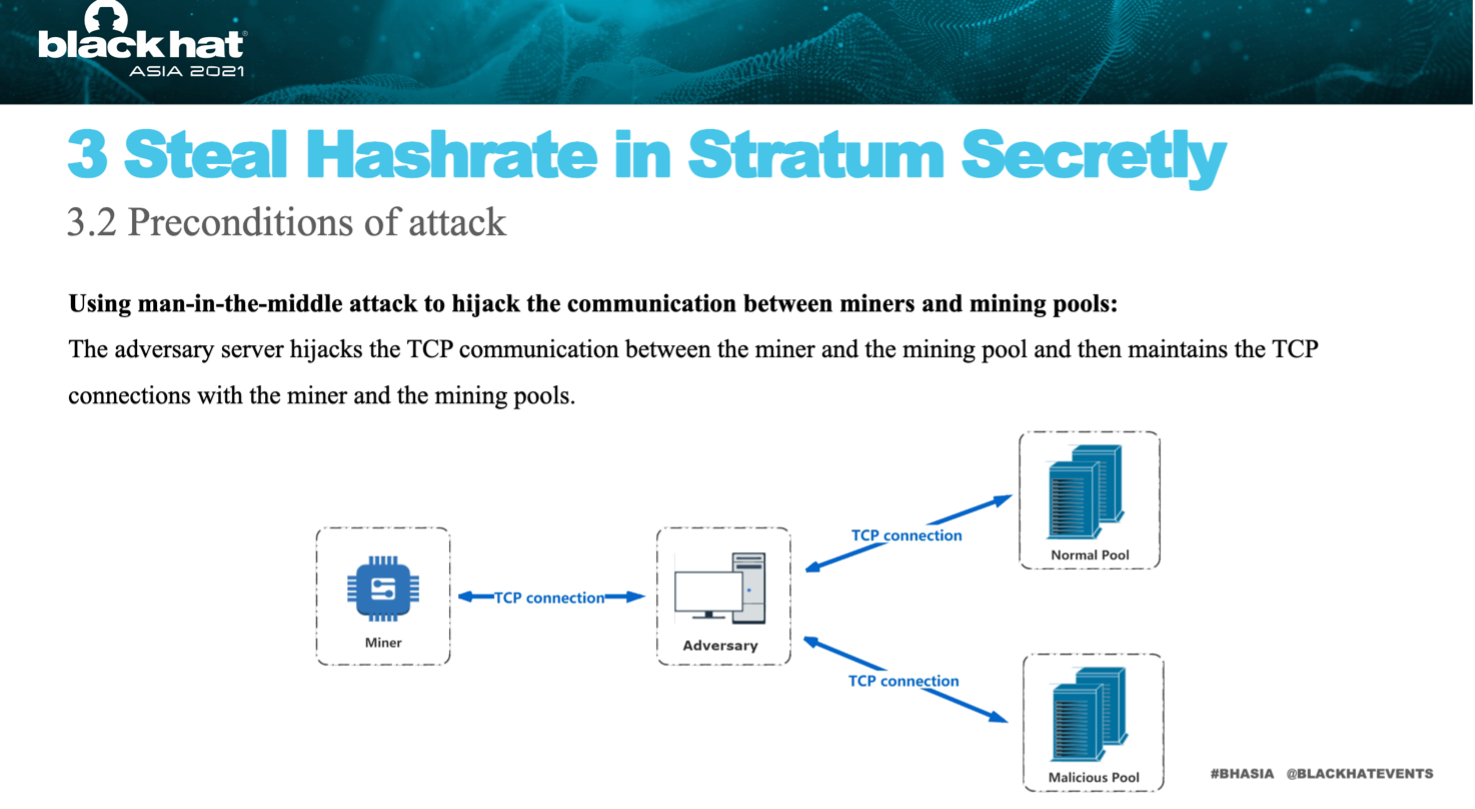
\includegraphics[width=15cm]{Figures/stratum/stratum4.png}
    \caption{Preconditions of attack, \textit{Blackhat Asia 2021}}
    \label{fig:stratum4}
\end{figure}

\noindent Given this precondition, the research group studied and analyzed two different possible attacks:
\begin{itemize}
    \item \textbf{Job injection based on set\_extranonce}
    \item \textbf{Time segment}
\end{itemize}

\subsubsection{\textbf{Job injection based on set\_extranonce}}
\noindent In the first attack scenario, basically the adversary firstly collects the subscription response of the two mining pool servers, saving locally the two couple of (entranonce1, extranonce2\_size).\\
At this point, the attacker sends to the miner the correct pool data, and he transfers all the future messages without changing them.\\
In the moment in which the adversary wants to steal the miner hashrate, he sends a set.extranonce message in which is put the "malicious" pool data (entranonce1, extranonce2\_size). 
Doing this, the miner will start working for the mining pool chosen by the attacker, without noticing it.

\begin{figure}[h!]
    \centering
    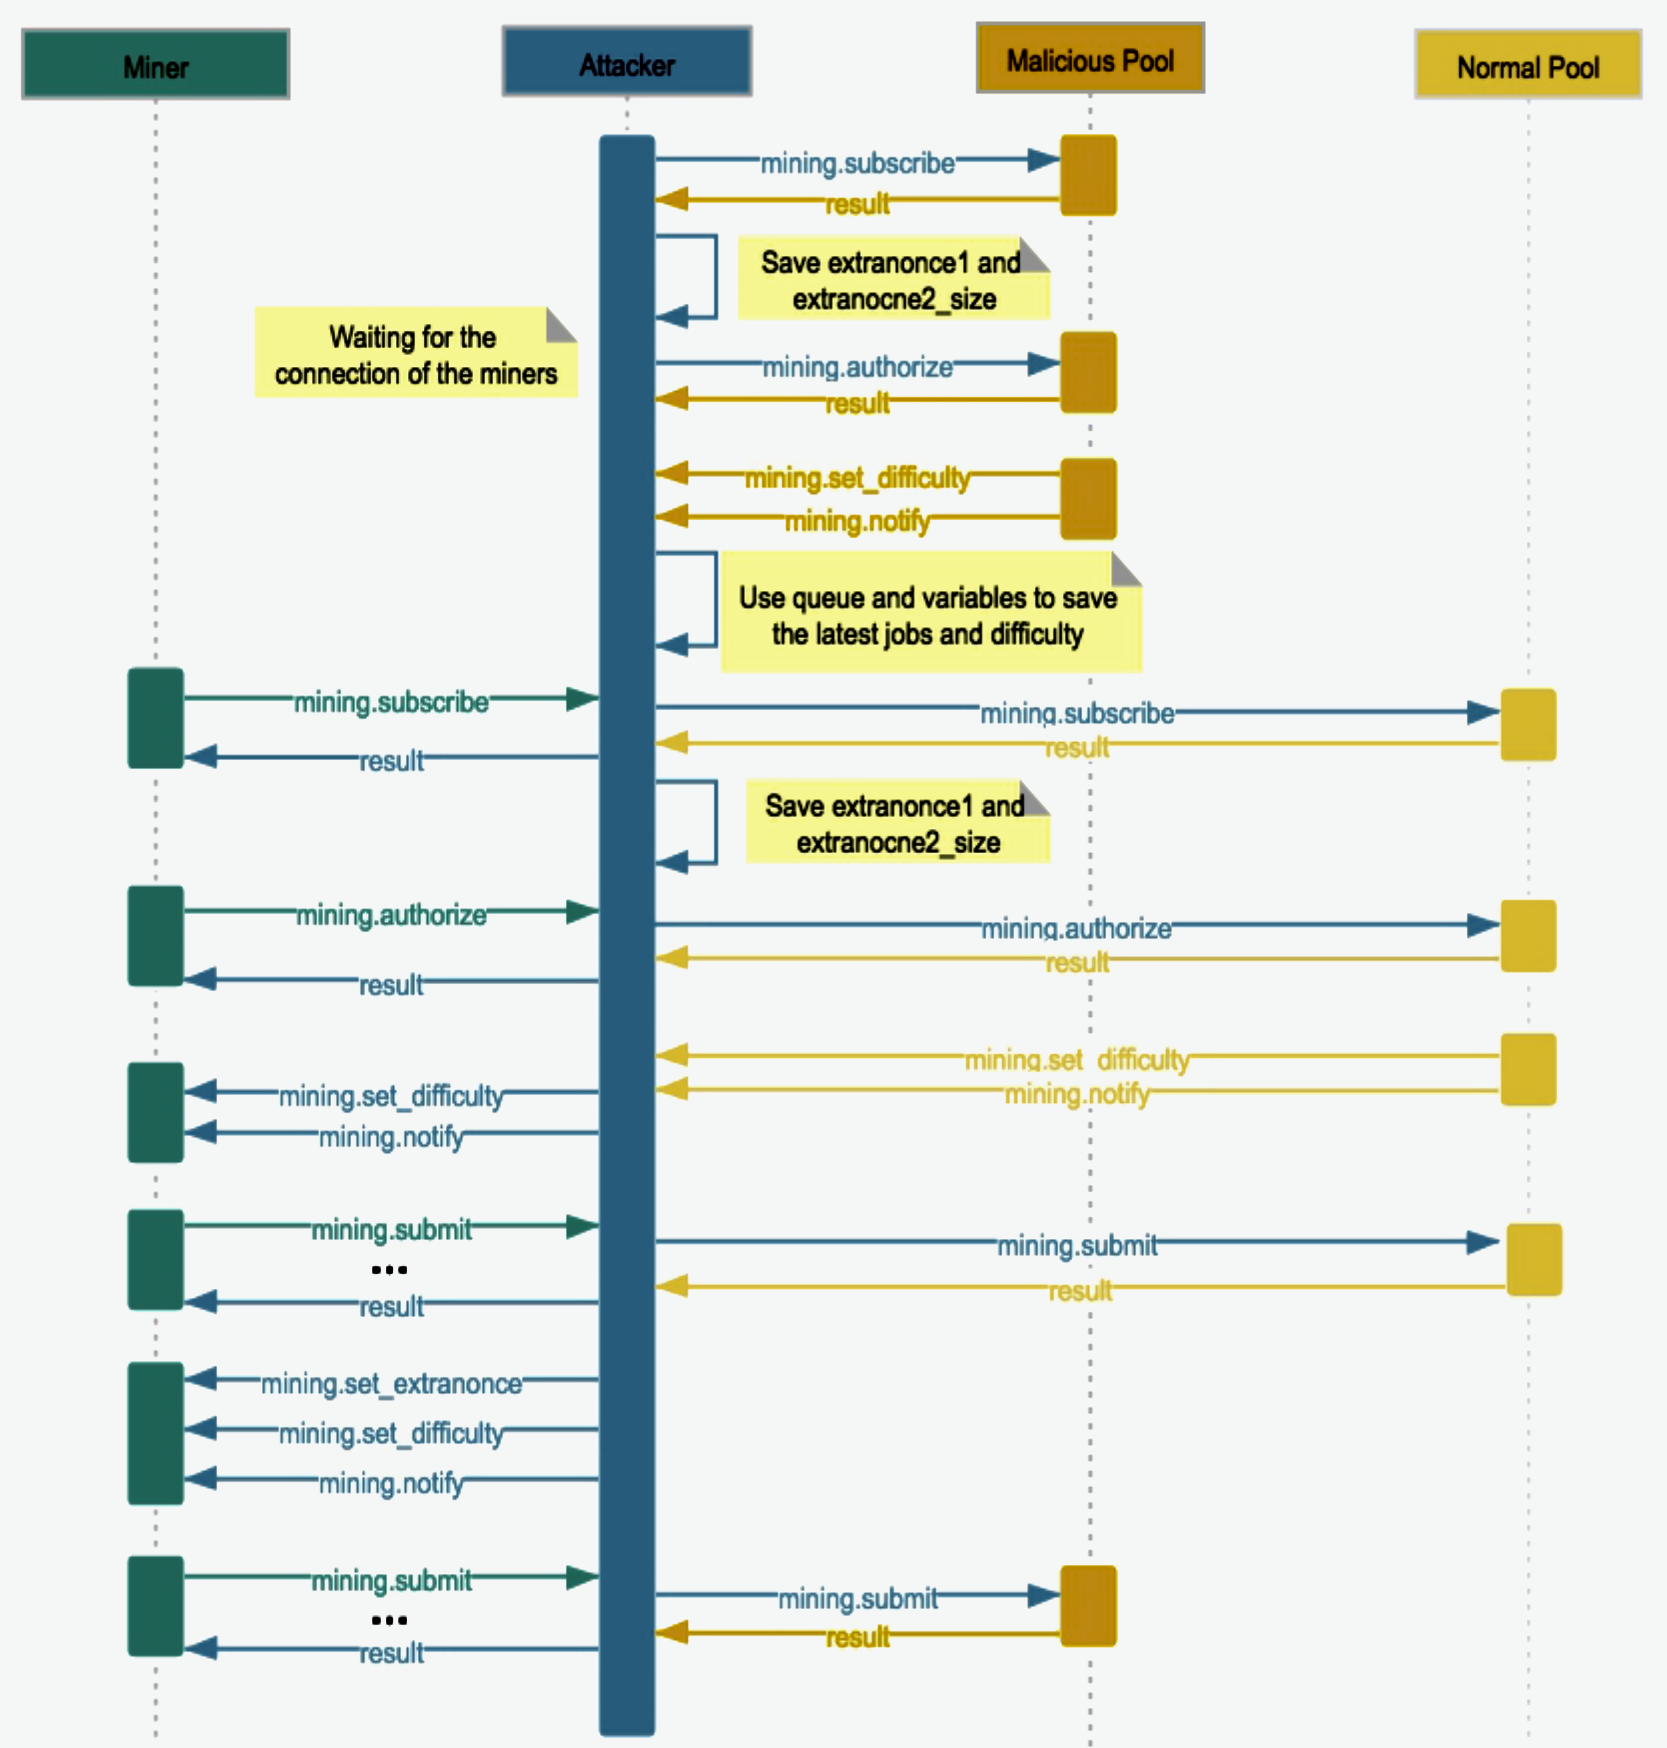
\includegraphics[width=14cm]{Figures/stratum/stratum5.png}
    \caption{Job injection based on set\_extranonce, \textit{Blackhat Asia 2021}}
    \label{fig:stratum5}
\end{figure}

\subsubsection{\textbf{Time segment}}
\noindent Regarding the second attack documented by the research group, it has some similarities to the previous one, but this time the client.reconnect message is used to ask the miner a re-connection to the "malicious" pool server, after a specific time segment.

\begin{figure}[h!]
    \centering
    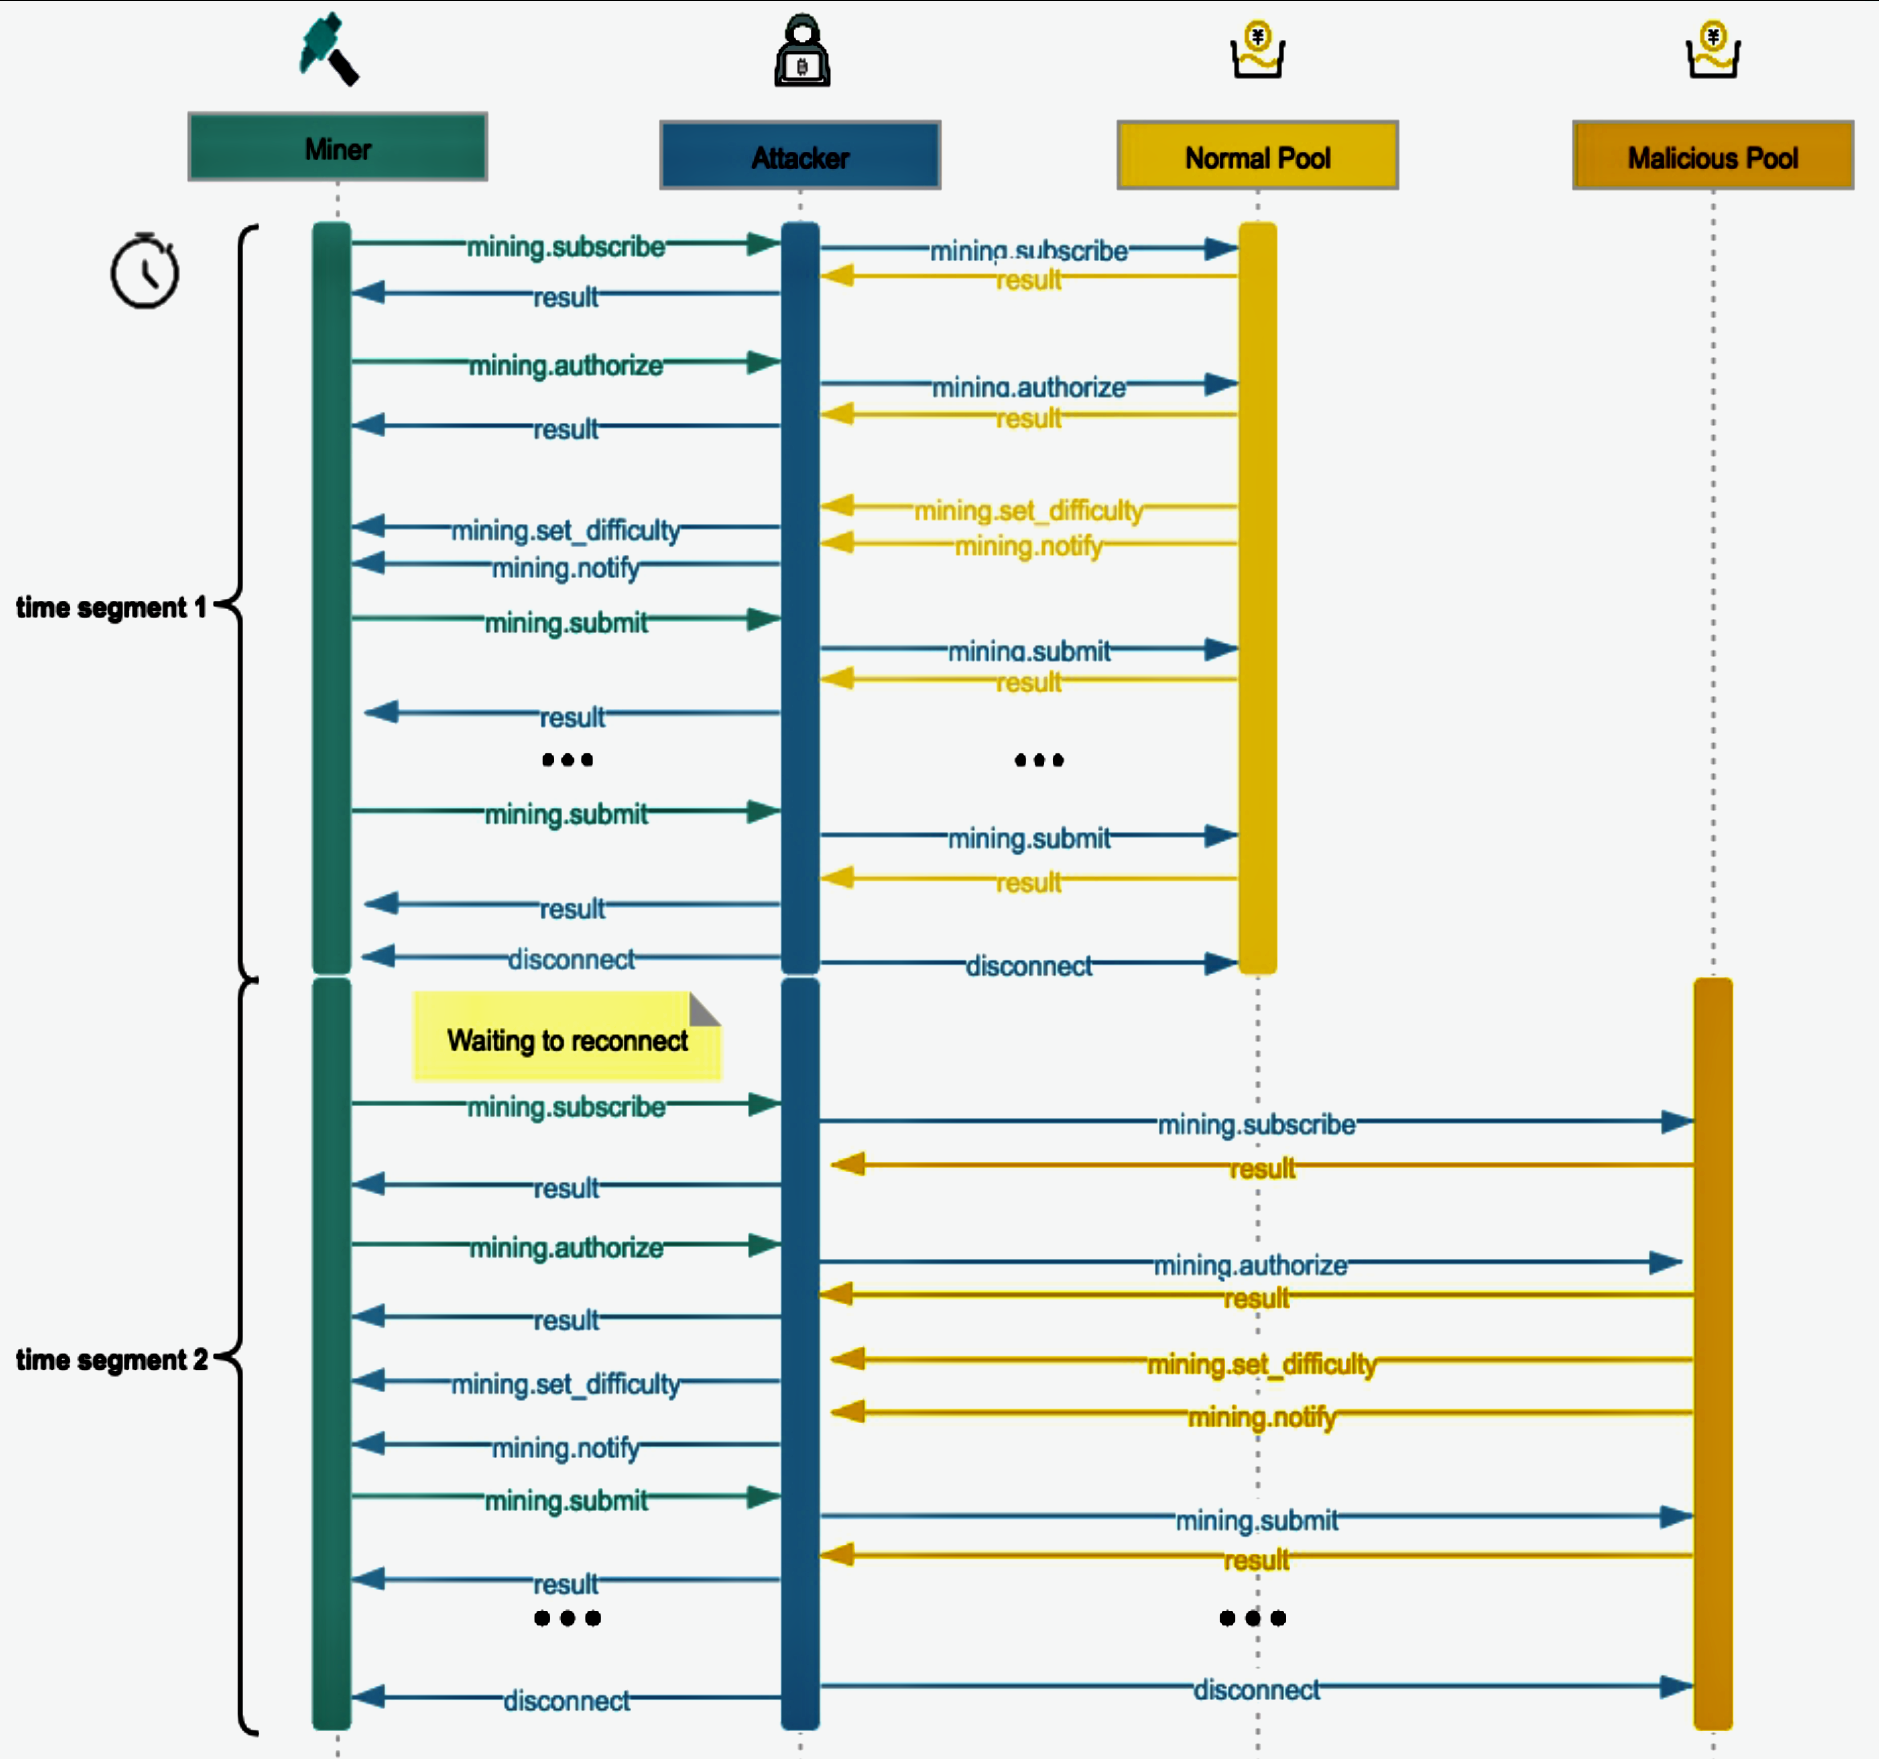
\includegraphics[width=15cm]{Figures/stratum/stratum6.png}
    \caption{Time segment attack, \textit{Blackhat Asia 2021}}
    \label{fig:stratum6}
\end{figure}

\noindent The job injection based on the set\_extranonce attack model provides better hiding aspect due to its ability to insert a small number of "malicious" mining pool jobs into the miner's job flow at a low frequency. This makes it difficult for the mining pool operator and the miner to detect the presence of the attack.\\
In the second attack model, the connection between the legitimate pool and the "malicious" pool is switched within specific time segments. In this way, the mining pool administrator may observe fluctuations in the overall computing power.\\\\
Both of the attack schemes described above are designed with the intention of illicitly stealing part of the miner hashrate, and both of them perfectly work.
To investigate more about the Proof of Concept done by the above-mentioned research group, some live-demonstration videos are available on Youtube. \cite{jobinjection}